\documentclass[11pt]{article}
\usepackage{amsmath,amssymb,amsthm}
\usepackage{geometry}
\usepackage{hyperref}

\geometry{margin=2.5cm}
\setlength{\parskip}{0.5em}
\setlength{\parindent}{0em}

\usepackage{tikz}
\usetikzlibrary{angles,fit,arrows,calc,math,matrix,intersections,through,backgrounds,cd}

\theoremstyle{definition}
\newtheorem{definition}{Definition}[section]

\title{A First Example of Arithmetic Loop and Conformal Handedness\\[0.3em]
  (Figure-eight knot and the two grids in $\mathfrak{E}_1$)}
\author{Mingli Yuan (draft note)}
\date{\today}

\begin{document}
\maketitle

\section{Setup: $\mathfrak{E}_1$, the assignment $a=-x/y$, and the figure-eight knot}

We work on the upper half-plane
\[
  \mathfrak{E}_1 = \{(x,y)\in\mathbb{R}^2 \mid y>0\}
\]
with the hyperbolic metric
\[
  ds^2 = \frac{dx^2 + dy^2}{y^2},
\]
and the assignment field
\[
  a(x,y) = -\frac{x}{y}.
\]
The level sets of $y$ and $x$ give the simplest ``rectangular'' arithmetic grid:
\begin{itemize}
  \item horizontal lines $y = \text{const}$ are \emph{addition lines};
  \item vertical lines $x = \text{const}$ are \emph{multiplication lines}.
\end{itemize}

We consider the figure-eight knot $4_1$, with group presentation
\[
  G(4_1) = \langle a,b \mid abbbaBAAB = 1 \rangle.
\]
Following the arithmetic expression interpretation, we map
\[
  a \mapsto \otimes t,\qquad b \mapsto \oplus 1,\qquad
  A = a^{-1} \mapsto \oslash t,\qquad B = b^{-1} \mapsto \ominus 1,
\]
so the relator
\[
  w := abbbaBAAB
\]
is interpreted as a threadlike expression in two generators $\oplus 1$ and $\otimes t$.

\begin{definition}[Loop (operator level)]
Let $\rho_t$ be the representation to affine maps $x\mapsto \Phi x + A$ induced by
\[
  \oplus 1: x \mapsto x+1,\qquad
  \otimes t: x \mapsto t x.
\]
A word $w$ in these generators is called an \emph{arithmetic loop} (at parameter $t$)
if the induced operator is the identity:
\[
  \rho_t(w) = \mathrm{Id}.
\]
\end{definition}

\section{The rectangular grid and the $4_1$ loop}

\subsection{Generator moves on the grid}

On the rectangular grid, a step of each generator acts on $(x,y)$ as follows:
\begin{align*}
  b = \oplus 1 &: \quad 
   a' = a+1 \iff (x',y')=(x-y,\ y),\\
  B = \ominus 1 &: \quad 
   a' = a-1 \iff (x',y')=(x+y,\ y),\\
  a = \otimes t &: \quad 
   a' = t\,a \iff (x',y')=(x,\ y/t),\\
  A = \oslash t &: \quad 
   a' = a/t \iff (x',y')=(x,\ y\,t).
\end{align*}
Thus,
\begin{itemize}
  \item $b,B$ move horizontally along an addition line;
  \item $a,A$ move vertically along a multiplication line.
\end{itemize}

We choose the basepoint
\[
  P_0 = (0,1) \quad (\text{so } a(P_0)=0).
\]

\subsection{Evaluating the relator as an operator}

As a function on $x$, the relator acts from right to left:
\[
  w(x) = a\bigl(b(b(b(a(B(A(A(B(x))))))))\bigr).
\]

Direct calculation gives
\begin{align*}
  B(x) &= x-1, \\
  A(B(x)) &= (x-1)t^{-1}, \\
  A(A(B(x))) &= (x-1)t^{-2}, \\
  B(A(A(B(x)))) &= (x-1)t^{-2} - 1, \\
  a(\cdot) &= t\cdot, \\
  b(\cdot) &= \cdot + 1.
\end{align*}
Carrying through the composition (as already checked in earlier computations) yields
\[
  w(x) = x - \bigl(t^2 - 3t + 1\bigr).
\]
Therefore $w$ is an operator-level loop if and only if
\[
  t^2 - 3t + 1 = 0,
\]
i.e.\ $t$ is a root of the Alexander polynomial $\Delta(t)=t^2-3t+1$ of $4_1$.

\subsection{The grid path for $w=abbbaBAAB$}

On the grid, the word $w=abbbaBAAB$ is read from right to left as the sequence
\[
  B, A, A, B, a, b, b, b, a.
\]

Starting from $P_0=(0,1)$, the successive points are:

\begin{align*}
  P_0 &= (0,1), \\
  P_1 = B(P_0) &= (0+1,\,1) = (1,1),\\
  P_2 = A(P_1) &= (1,\,1\cdot t) = (1,t),\\
  P_3 = A(P_2) &= (1,\,t^2),\\
  P_4 = B(P_3) &= (1+t^2,\,t^2),\\
  P_5 = a(P_4) &= (1+t^2,\,t),\\
  P_6 = b(P_5) &= (1+t^2 - t,\,t),\\
  P_7 = b(P_6) &= (1+t^2 - 2t,\,t),\\
  P_8 = b(P_7) &= (1+t^2 - 3t,\,t),\\
  P_9 = a(P_8) &= (1+t^2 - 3t,\,1).
\end{align*}

Thus the path is closed on the rectangular grid if and only if
\[
  P_9 = P_0 \iff 1+t^2-3t=0 \iff t^2-3t+1=0.
\]
On exactly the same condition where the operator becomes the identity, the geometric path is a loop.

\begin{figure}[h]
  \centering
  \includegraphics[width=0.6\textwidth]{images/knot_4_1.pdf}
  \caption{The loop $abbbaBAAB$ of the figure-eight knot on the first (rectangular)
    arithmetic grid in $\mathfrak{E}_1$.}
\end{figure}

\section{The curved grid via $w=-1/z$ and the same assignment $a=-x/y$}

Now consider the conformal map
\[
  w = u+iv = -\frac{1}{z} = -\frac{1}{x+iy}
    = \left(-\frac{x}{x^2+y^2},\ \frac{y}{x^2+y^2}\right).
\]

On the same $(x,y)$-plane, we can draw a second grid:

\begin{itemize}
  \item \textbf{blue family}: circles with centre on the $y$-axis, radii
    $R\in\{1/2,1,2,4,8\}$:
    \[
      B_R:\quad x^2 + (y-R)^2 = R^2;
    \]
  \item \textbf{green family}: circles with centre on the $x$-axis, radii
    $r\in\{1/2,1,2,4,8\}$:
    \[
      G_{r,c}:\quad (x-c)^2 + y^2 = r^2,\quad c=\pm r.
    \]
\end{itemize}

These are exactly the images of horizontal and vertical lines under $w=-1/z$ (viewed back in the original coordinate system). They form a curved arithmetic grid.

\begin{figure}[h]
  \centering
  % this is exactly your 18-grid-example-2.tex code, adapted to be inside a figure
  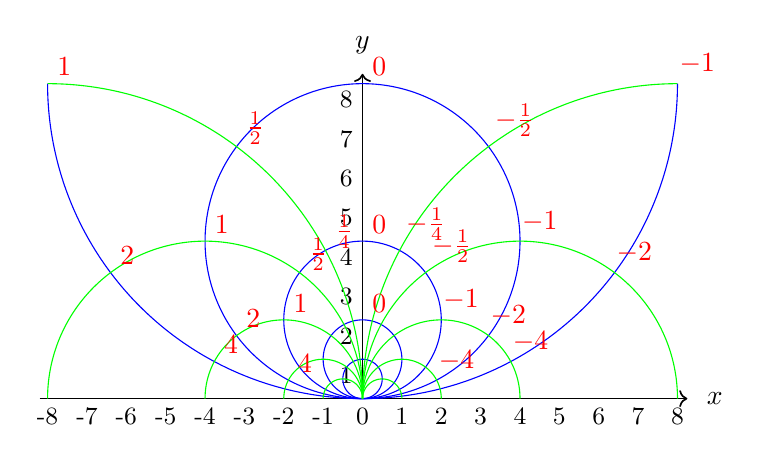
\begin{tikzpicture}[scale=0.5]
    \draw [black, line width=0.6pt, ->] (0,0) -- (0,8.25);
    \node [anchor=south] at (0,8.5) {$y$};
    \draw [black, line width=0.6pt, ->] (-8.2,0) -- (8.25,0);
    \node [anchor=west] at (8.5,0) {$x$};
    \foreach \x in {-8,-7,-6,-5,-4,-3,-2,-1,0,1,2,3,4,5,6,7,8}
      \node [anchor=north] at (\x,0) {\small \x};
    \foreach \y in {1,2,3,4,5,6,7,8}
      \node [anchor=45] at (0,\y) {\small \y};

    % blue circles
    \draw[blue,scale=1.0,samples=360,domain=0.0:360,variable=\t] 
      plot ({0.5 * cos(\t) },{0.5 + 0.5 * sin(\t)});
    \draw[blue,scale=1.0,samples=360,domain=0.0:360,variable=\t] 
      plot ({1 * cos(\t) },{1 + 1 * sin(\t)});
    \draw[blue,scale=1.0,samples=360,domain=0.0:360,variable=\t] 
      plot ({2 * cos(\t) },{2 + 2 * sin(\t)});
    \draw[blue,scale=1.0,samples=360,domain=0.0:360,variable=\t] 
      plot ({4 * cos(\t) },{4 + 4 * sin(\t)});
    \draw[blue,scale=1.0,samples=360,domain=-180:0.0,variable=\t] 
      plot ({8 * cos(\t) },{8 + 8 * sin(\t)});

    % green circles (right)
    \draw[green,scale=1.0,samples=360,domain=0.0:180,variable=\t] 
      plot ({0.5 + 0.5 * cos(\t) },{0.5 * sin(\t)});
    \draw[green,scale=1.0,samples=360,domain=0.0:180,variable=\t] 
      plot ({1 + 1 * cos(\t) },{1 * sin(\t)});
    \draw[green,scale=1.0,samples=360,domain=0.0:180,variable=\t] 
      plot ({2 + 2 * cos(\t) },{2 * sin(\t)});
    \draw[green,scale=1.0,samples=360,domain=0.0:180,variable=\t] 
      plot ({4 + 4 * cos(\t) },{4 * sin(\t)});
    \draw[green,scale=1.0,samples=360,domain=90:180,variable=\t] 
      plot ({8 + 8 * cos(\t) },{8 * sin(\t)});

    % green circles (left)
    \draw[green,scale=1.0,samples=360,domain=0.0:180,variable=\t] 
      plot ({-0.5 + 0.5 * cos(\t) },{0.5 * sin(\t)});
    \draw[green,scale=1.0,samples=360,domain=0.0:180,variable=\t] 
      plot ({-1 + 1 * cos(\t) },{1 * sin(\t)});
    \draw[green,scale=1.0,samples=360,domain=0.0:180,variable=\t] 
      plot ({-2 + 2 * cos(\t) },{2 * sin(\t)});
    \draw[green,scale=1.0,samples=360,domain=0.0:180,variable=\t] 
      plot ({-4 + 4 * cos(\t) },{4 * sin(\t)});
    \draw[green,scale=1.0,samples=360,domain=0.0:90.0,variable=\t] 
      plot ({-8 + 8 * cos(\t) },{8 * sin(\t)});

    % sample labels for a = -x/y
    \node [anchor=225, red] at (64/17, 16/17) {$-4$};
    \node [anchor=225, red] at (32/5, 16/5) {$-2$};
    \node [anchor=225, red] at (8, 8) {$-1$};
    \node [anchor=225, red] at (-8, 8) {$1$};
    \node [anchor=225, red] at (-32/5, 16/5) {$2$};
    \node [anchor=225, red] at (-64/17, 16/17) {$4$};

    \node [anchor=225, red] at (32/17, 8/17) {$-4$};
    \node [anchor=225, red] at (16/5, 8/5) {$-2$};
    \node [anchor=225, red] at (4, 4) {$-1$};
    \node [anchor=225, red] at (16/5, 32/5) {$-\tfrac{1}{2}$};
    \node [anchor=225, red] at (0, 8) {$0$};
    \node [anchor=225, red] at (-16/5, 32/5) {$\tfrac{1}{2}$};
    \node [anchor=225, red] at (-4, 4) {$1$};
    \node [anchor=225, red] at (-16/5, 8/5) {$2$};
    \node [anchor=225, red] at (-32/17, 8/17) {$4$};

    \node [anchor=225, red] at (2, 2) {$-1$};
    \node [anchor=225, red] at (8/5, 16/5) {$-\tfrac{1}{2}$};
    \node [anchor=225, red] at (16/17, 64/17) {$-\tfrac{1}{4}$};
    \node [anchor=225, red] at (0, 4) {$0$};
    \node [anchor=225, red] at (-16/17, 64/17) {$\tfrac{1}{4}$}; % sign corrected
    \node [anchor=225, red] at (-8/5, 16/5) {$\tfrac{1}{2}$};
    \node [anchor=225, red] at (-2, 2) {$1$};

    \node [anchor=225, red] at (0, 2) {$0$};

  \end{tikzpicture}
  \caption{Curved grid in the same $\mathfrak{E}_1$ with the same assignment $a=-x/y$.}
\end{figure}

\subsection{Intersection coordinates and the same assignment}

Let $B_R$ be a blue circle of radius $R$, centred at $(0,R)$, and let
$G_{r,c}$ be a green circle of radius $r$, centred at $(c,0)$ with $c=\pm r$.
Their intersection in the upper half-plane (excluding the origin) is at
\[
  (x,y) = \left(
    \frac{2R^2 r}{R^2+r^2}\,\operatorname{sign}(c),\ 
    \frac{2R r^2}{R^2+r^2}
  \right).
\]
At this point, the assignment value is
\[
  a = -\frac{x}{y} = -\frac{R}{c} = \mp\frac{R}{r}.
\]
Thus all red labels in the curved grid are still given by the same field
$a=-x/y$ evaluated at different intersection points of blue/green circles.

\section{Handedness flip and the loop under $w=-1/z$}

The conformal map $w=-1/z$ is orientation-reversing on the upper half-plane.
At the level of grids:

\begin{itemize}
  \item horizontal (addition) lines and vertical (multiplication) lines are
        sent to the two orthogonal families of circles described above;
  \item the assignment field transforms as
        $a(x,y)=-x/y \mapsto a(w) = -u/v = -a(z)$, i.e.\ it flips sign,
        but in our curved grid construction we re-interpret the sign via 
        a handedness convention for addition/multiplication directions.
\end{itemize}

Conceptually,
\begin{itemize}
  \item the rectangular grid realises $\oplus1$ and $\otimes t$ along straight
        axes, with one choice of handedness;
  \item the curved grid realises the \emph{same arithmetic field} $a=-x/y$
        and the \emph{same loop} at the operator level, but in a different
        geometric chart where the local frame of
        \[
          (\text{``add one'' direction},\ \text{``multiply by $t$'' direction})
        \]
        has opposite chirality.
\end{itemize}

Given a loop $L$ (for example, the geometric path of $w=abbbaBAAB$ in the
rectangular grid):
\begin{itemize}
  \item applying $w=-1/z$ to the path only produces a new curve $L'$ in the
        same background $(\mathfrak{E}_1,a=-x/y)$;
  \item by construction of the curved grid, $L'$ can still be read as a
        threadlike expression in $\oplus1,\otimes t$ (now along circles);
  \item reversing the parametrisation of $L'$ corresponds to the inverse word
        $w^{-1}$; but since $\rho_t(w)=\mathrm{Id}$ we also have
        $\rho_t(w^{-1})=\mathrm{Id}$, so $L'$ with reversed orientation is
        again an arithmetic loop.
\end{itemize}

In this way, the symmetry of the Alexander polynomial $\Delta(t)$ under
$t\leftrightarrow t^{-1}$, the amphicheiral nature of the figure-eight knot,
and the geometric handedness flip induced by $w=-1/z$ are all reflected in
the same picture of loops in $\mathfrak{E}_1$.

\section{Remarks and next steps}

This note only records one concrete example:
\begin{itemize}
  \item an operator-level loop $w$ coming from a knot relator and its Alexander
        polynomial;
  \item its realisation as a geometric loop in the rectangular arithmetic grid;
  \item the conformal image of this loop under $w=-1/z$ and its re-reading
        in the curved arithmetic grid on the same assignment field.
\end{itemize}

The general theory of \emph{free loops} --- loops not tied to a specific
grid, but living in the background $(\mathfrak{E}_1,a)$ and its conformal
self-maps --- will be developed in a subsequent note.

\end{document}
